\documentclass[1p]{elsarticle_modified}
%\bibliographystyle{elsarticle-num}

%\usepackage[colorlinks]{hyperref}
%\usepackage{abbrmath_seonhwa} %\Abb, \Ascr, \Acal ,\Abf, \Afrak
\usepackage{amsfonts}
\usepackage{amssymb}
\usepackage{amsmath}
\usepackage{amsthm}
\usepackage{scalefnt}
\usepackage{amsbsy}
\usepackage{kotex}
\usepackage{caption}
\usepackage{subfig}
\usepackage{color}
\usepackage{graphicx}
\usepackage{xcolor} %% white, black, red, green, blue, cyan, magenta, yellow
\usepackage{float}
\usepackage{setspace}
\usepackage{hyperref}

\usepackage{tikz}
\usetikzlibrary{arrows}

\usepackage{multirow}
\usepackage{array} % fixed length table
\usepackage{hhline}

%%%%%%%%%%%%%%%%%%%%%
\makeatletter
\renewcommand*\env@matrix[1][\arraystretch]{%
	\edef\arraystretch{#1}%
	\hskip -\arraycolsep
	\let\@ifnextchar\new@ifnextchar
	\array{*\c@MaxMatrixCols c}}
\makeatother %https://tex.stackexchange.com/questions/14071/how-can-i-increase-the-line-spacing-in-a-matrix
%%%%%%%%%%%%%%%

\usepackage[normalem]{ulem}

\newcommand{\msout}[1]{\ifmmode\text{\sout{\ensuremath{#1}}}\else\sout{#1}\fi}
%SOURCE: \msout is \stkout macro in https://tex.stackexchange.com/questions/20609/strikeout-in-math-mode

\newcommand{\cancel}[1]{
	\ifmmode
	{\color{red}\msout{#1}}
	\else
	{\color{red}\sout{#1}}
	\fi
}

\newcommand{\add}[1]{
	{\color{blue}\uwave{#1}}
}

\newcommand{\replace}[2]{
	\ifmmode
	{\color{red}\msout{#1}}{\color{blue}\uwave{#2}}
	\else
	{\color{red}\sout{#1}}{\color{blue}\uwave{#2}}
	\fi
}

\newcommand{\Sol}{\mathcal{S}} %segment
\newcommand{\D}{D} %diagram
\newcommand{\A}{\mathcal{A}} %arc


%%%%%%%%%%%%%%%%%%%%%%%%%%%%%5 test

\def\sl{\operatorname{\textup{SL}}(2,\Cbb)}
\def\psl{\operatorname{\textup{PSL}}(2,\Cbb)}
\def\quan{\mkern 1mu \triangleright \mkern 1mu}

\theoremstyle{definition}
\newtheorem{thm}{Theorem}[section]
\newtheorem{prop}[thm]{Proposition}
\newtheorem{lem}[thm]{Lemma}
\newtheorem{ques}[thm]{Question}
\newtheorem{cor}[thm]{Corollary}
\newtheorem{defn}[thm]{Definition}
\newtheorem{exam}[thm]{Example}
\newtheorem{rmk}[thm]{Remark}
\newtheorem{alg}[thm]{Algorithm}

\newcommand{\I}{\sqrt{-1}}
\begin{document}

%\begin{frontmatter}
%
%\title{Boundary parabolic representations of knots up to 8 crossings}
%
%%% Group authors per affiliation:
%\author{Yunhi Cho} 
%\address{Department of Mathematics, University of Seoul, Seoul, Korea}
%\ead{yhcho@uos.ac.kr}
%
%
%\author{Seonhwa Kim} %\fnref{s_kim}}
%\address{Center for Geometry and Physics, Institute for Basic Science, Pohang, 37673, Korea}
%\ead{ryeona17@ibs.re.kr}
%
%\author{Hyuk Kim}
%\address{Department of Mathematical Sciences, Seoul National University, Seoul 08826, Korea}
%\ead{hyukkim@snu.ac.kr}
%
%\author{Seokbeom Yoon}
%\address{Department of Mathematical Sciences, Seoul National University, Seoul, 08826,  Korea}
%\ead{sbyoon15@snu.ac.kr}
%
%\begin{abstract}
%We find all boundary parabolic representation of knots up to 8 crossings.
%
%\end{abstract}
%\begin{keyword}
%    \MSC[2010] 57M25 
%\end{keyword}
%
%\end{frontmatter}

%\linenumbers
%\tableofcontents
%
\newcommand\colored[1]{\textcolor{white}{\rule[-0.35ex]{0.8em}{1.4ex}}\kern-0.8em\color{red} #1}%
%\newcommand\colored[1]{\textcolor{white}{ #1}\kern-2.17ex	\textcolor{white}{ #1}\kern-1.81ex	\textcolor{white}{ #1}\kern-2.15ex\color{red}#1	}

{\Large $\underline{12n_{0598}~(K12n_{0598})}$}

\setlength{\tabcolsep}{10pt}
\renewcommand{\arraystretch}{1.6}
\vspace{1cm}\begin{tabular}{m{100pt}>{\centering\arraybackslash}m{274pt}}
\multirow{5}{120pt}{
	\centering
	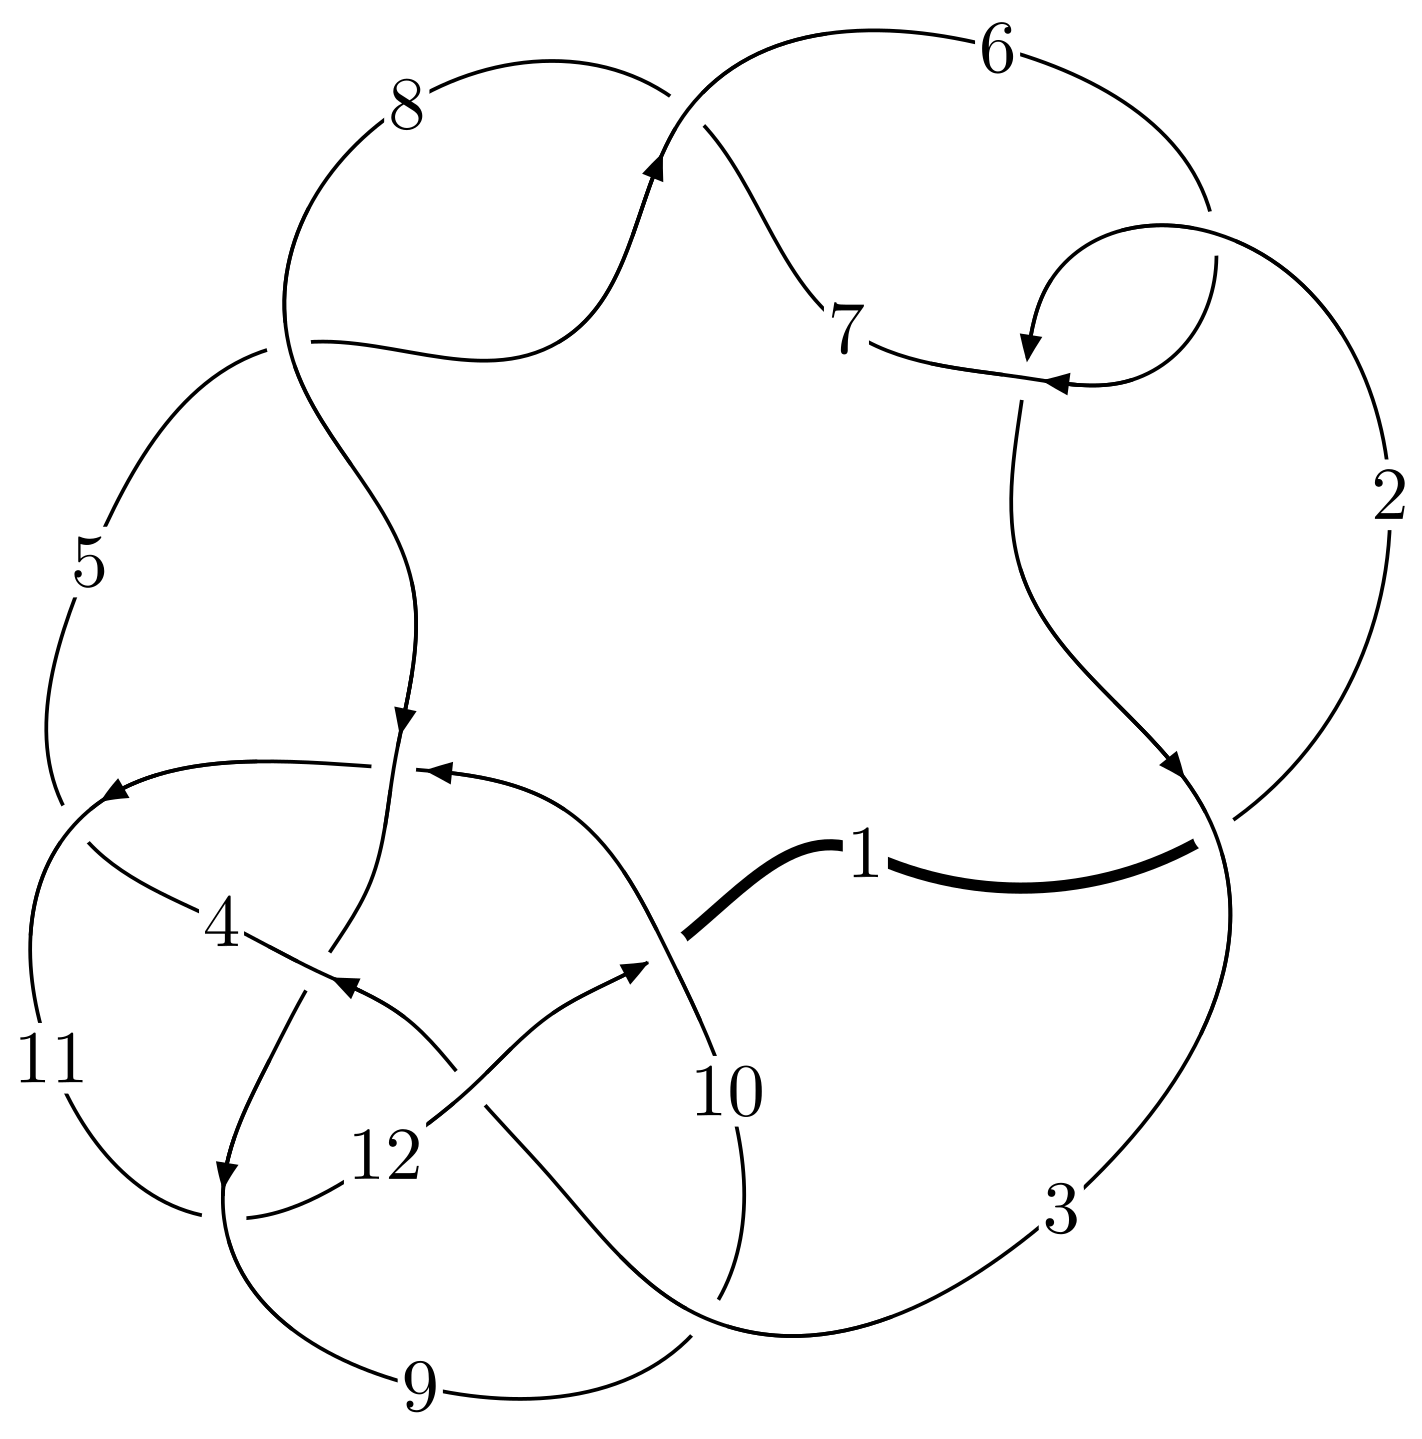
\includegraphics[width=112pt]{../../../GIT/diagram.site/Diagrams/png/2687_12n_0598.png}\\
\ \ \ A knot diagram\footnotemark}&
\allowdisplaybreaks
\textbf{Linearized knot diagam} \\
\cline{2-2}
 &
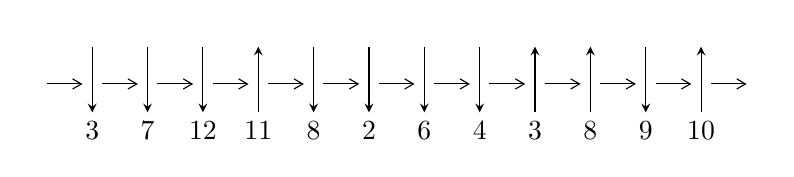
\begin{tikzpicture}[x=20pt, y=17pt]
	% nodes
	\node (C0) at (0, 0) {};
	\node (C1) at (1, 0) {};
	\node (C1U) at (1, +1) {};
	\node (C1D) at (1, -1) {3};

	\node (C2) at (2, 0) {};
	\node (C2U) at (2, +1) {};
	\node (C2D) at (2, -1) {7};

	\node (C3) at (3, 0) {};
	\node (C3U) at (3, +1) {};
	\node (C3D) at (3, -1) {12};

	\node (C4) at (4, 0) {};
	\node (C4U) at (4, +1) {};
	\node (C4D) at (4, -1) {11};

	\node (C5) at (5, 0) {};
	\node (C5U) at (5, +1) {};
	\node (C5D) at (5, -1) {8};

	\node (C6) at (6, 0) {};
	\node (C6U) at (6, +1) {};
	\node (C6D) at (6, -1) {2};

	\node (C7) at (7, 0) {};
	\node (C7U) at (7, +1) {};
	\node (C7D) at (7, -1) {6};

	\node (C8) at (8, 0) {};
	\node (C8U) at (8, +1) {};
	\node (C8D) at (8, -1) {4};

	\node (C9) at (9, 0) {};
	\node (C9U) at (9, +1) {};
	\node (C9D) at (9, -1) {3};

	\node (C10) at (10, 0) {};
	\node (C10U) at (10, +1) {};
	\node (C10D) at (10, -1) {8};

	\node (C11) at (11, 0) {};
	\node (C11U) at (11, +1) {};
	\node (C11D) at (11, -1) {9};

	\node (C12) at (12, 0) {};
	\node (C12U) at (12, +1) {};
	\node (C12D) at (12, -1) {10};
	\node (C13) at (13, 0) {};

	% arrows
	\draw[->,>={angle 60}]
	(C0) edge (C1) (C1) edge (C2) (C2) edge (C3) (C3) edge (C4) (C4) edge (C5) (C5) edge (C6) (C6) edge (C7) (C7) edge (C8) (C8) edge (C9) (C9) edge (C10) (C10) edge (C11) (C11) edge (C12) (C12) edge (C13) ;	\draw[->,>=stealth]
	(C1U) edge (C1D) (C2U) edge (C2D) (C3U) edge (C3D) (C4D) edge (C4U) (C5U) edge (C5D) (C6U) edge (C6D) (C7U) edge (C7D) (C8U) edge (C8D) (C9D) edge (C9U) (C10D) edge (C10U) (C11U) edge (C11D) (C12D) edge (C12U) ;
	\end{tikzpicture} \\
\hhline{~~} \\& 
\textbf{Solving Sequence} \\ \cline{2-2} 
 &
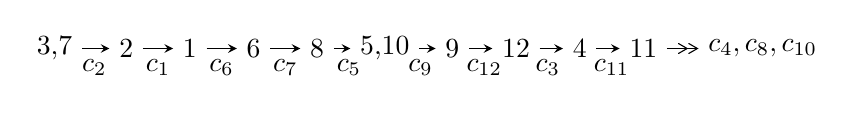
\begin{tikzpicture}[x=23pt, y=7pt]
	% node
	\node (A0) at (-1/8, 0) {3,7};
	\node (A1) at (1, 0) {2};
	\node (A2) at (2, 0) {1};
	\node (A3) at (3, 0) {6};
	\node (A4) at (4, 0) {8};
	\node (A5) at (81/16, 0) {5,10};
	\node (A6) at (49/8, 0) {9};
	\node (A7) at (57/8, 0) {12};
	\node (A8) at (65/8, 0) {4};
	\node (A9) at (73/8, 0) {11};
	\node (C1) at (1/2, -1) {$c_{2}$};
	\node (C2) at (3/2, -1) {$c_{1}$};
	\node (C3) at (5/2, -1) {$c_{6}$};
	\node (C4) at (7/2, -1) {$c_{7}$};
	\node (C5) at (9/2, -1) {$c_{5}$};
	\node (C6) at (45/8, -1) {$c_{9}$};
	\node (C7) at (53/8, -1) {$c_{12}$};
	\node (C8) at (61/8, -1) {$c_{3}$};
	\node (C9) at (69/8, -1) {$c_{11}$};
	\node (A10) at (11, 0) {$c_{4},c_{8},c_{10}$};

	% edge
	\draw[->,>=stealth]	
	(A0) edge (A1) (A1) edge (A2) (A2) edge (A3) (A3) edge (A4) (A4) edge (A5) (A5) edge (A6) (A6) edge (A7) (A7) edge (A8) (A8) edge (A9) ;
	\draw[->>,>={angle 60}]	
	(A9) edge (A10);
\end{tikzpicture} \\ 

\end{tabular} \\

\footnotetext{
The image of knot diagram is generated by the software ``\textbf{Draw programme}" developed by Andrew Bartholomew(\url{http://www.layer8.co.uk/maths/draw/index.htm\#Running-draw}), where we modified some parts for our purpose(\url{https://github.com/CATsTAILs/LinksPainter}).
}\phantom \\ \newline 
\centering \textbf{Ideals for irreducible components\footnotemark of $X_{\text{par}}$} 
 
\begin{align*}
I^u_{1}&=\langle 
-7 u^{26}+30 u^{25}+\cdots+b+25,\;-17 u^{26}+93 u^{25}+\cdots+4 a+113,\;u^{27}-5 u^{26}+\cdots-21 u+4\rangle \\
I^u_{2}&=\langle 
u^{17}+2 u^{16}+\cdots+b- u,\;-2 u^{18}-2 u^{17}+\cdots- a+1,\;u^{19}+2 u^{18}+\cdots-2 u-1\rangle \\
I^u_{3}&=\langle 
- u^9+u^8+u^7-3 u^6- u^5+3 u^4- u^3- u^2+b- u,\\
\phantom{I^u_{3}}&\phantom{= \langle  }-3 u^9+3 u^8+4 u^7-9 u^6-4 u^5+11 u^4-6 u^2+a-2 u+2,\\
\phantom{I^u_{3}}&\phantom{= \langle  }u^{10}-2 u^9+4 u^7-2 u^6-4 u^5+4 u^4+u^3- u^2- u+1\rangle \\
I^u_{4}&=\langle 
u^2 a+a u- u^2+b- u-1,\;- u^2 a+a^2-2 a u+2 u^2- a+u+1,\;u^3+u^2-1\rangle \\
\\
\end{align*}
\raggedright * 4 irreducible components of $\dim_{\mathbb{C}}=0$, with total 81 representations.\\
\footnotetext{All coefficients of polynomials are rational numbers. But the coefficients are sometimes approximated in decimal forms when there is not enough margin.}
\newpage
\renewcommand{\arraystretch}{1}
\centering \section*{I. $I^u_{1}= \langle -7 u^{26}+30 u^{25}+\cdots+b+25,\;-17 u^{26}+93 u^{25}+\cdots+4 a+113,\;u^{27}-5 u^{26}+\cdots-21 u+4 \rangle$}
\flushleft \textbf{(i) Arc colorings}\\
\begin{tabular}{m{7pt} m{180pt} m{7pt} m{180pt} }
\flushright $a_{3}=$&$\begin{pmatrix}1\\0\end{pmatrix}$ \\
\flushright $a_{7}=$&$\begin{pmatrix}0\\u\end{pmatrix}$ \\
\flushright $a_{2}=$&$\begin{pmatrix}1\\- u^2\end{pmatrix}$ \\
\flushright $a_{1}=$&$\begin{pmatrix}- u^2+1\\- u^2\end{pmatrix}$ \\
\flushright $a_{6}=$&$\begin{pmatrix}u\\- u^3+u\end{pmatrix}$ \\
\flushright $a_{8}=$&$\begin{pmatrix}- u^3\\u^5- u^3+u\end{pmatrix}$ \\
\flushright $a_{5}=$&$\begin{pmatrix}u^5+u\\- u^7+u^5-2 u^3+u\end{pmatrix}$ \\
\flushright $a_{10}=$&$\begin{pmatrix}4.25000 u^{26}-23.2500 u^{25}+\cdots+127.250 u-28.2500\\7 u^{26}-30 u^{25}+\cdots+120 u-25\end{pmatrix}$ \\
\flushright $a_{9}=$&$\begin{pmatrix}-2.75000 u^{26}+6.75000 u^{25}+\cdots+7.25000 u-3.25000\\7 u^{26}-30 u^{25}+\cdots+120 u-25\end{pmatrix}$ \\
\flushright $a_{12}=$&$\begin{pmatrix}-\frac{1}{4} u^{26}-\frac{7}{4} u^{25}+\cdots+\frac{35}{4} u+\frac{1}{4}\\4 u^{26}-17 u^{25}+\cdots+56 u-11\end{pmatrix}$ \\
\flushright $a_{4}=$&$\begin{pmatrix}\frac{23}{4} u^{26}-\frac{95}{4} u^{25}+\cdots+\frac{295}{4} u-\frac{55}{4}\\4 u^{26}-14 u^{25}+\cdots+23 u-3\end{pmatrix}$ \\
\flushright $a_{11}=$&$\begin{pmatrix}-3.75000 u^{26}+11.7500 u^{25}+\cdots-16.7500 u+3.75000\\5 u^{26}-24 u^{25}+\cdots+109 u-25\end{pmatrix}$\\&\end{tabular}
\flushleft \textbf{(ii) Obstruction class $= -1$}\\~\\
\flushleft \textbf{(iii) Cusp Shapes $= 19 u^{26}-78 u^{25}+60 u^{24}+252 u^{23}-548 u^{22}-79 u^{21}+1369 u^{20}-955 u^{19}-1968 u^{18}+3221 u^{17}+1042 u^{16}-5938 u^{15}+2926 u^{14}+5761 u^{13}-7754 u^{12}-727 u^{11}+8181 u^{10}-4909 u^9-3262 u^8+5571 u^7-1366 u^6-2297 u^5+2086 u^4-317 u^3-482 u^2+330 u-70$}\\~\\
\newpage\renewcommand{\arraystretch}{1}
\flushleft \textbf{(iv) u-Polynomials at the component}\newline \\
\begin{tabular}{m{50pt}|m{274pt}}
Crossings & \hspace{64pt}u-Polynomials at each crossing \\
\hline $$\begin{aligned}c_{1},c_{5},c_{7}\end{aligned}$$&$\begin{aligned}
&u^{27}+11 u^{26}+\cdots+113 u+16
\end{aligned}$\\
\hline $$\begin{aligned}c_{2},c_{6}\end{aligned}$$&$\begin{aligned}
&u^{27}-5 u^{26}+\cdots-21 u+4
\end{aligned}$\\
\hline $$\begin{aligned}c_{3},c_{8}\end{aligned}$$&$\begin{aligned}
&u^{27}- u^{26}+\cdots+u+1
\end{aligned}$\\
\hline $$\begin{aligned}c_{4},c_{9}\end{aligned}$$&$\begin{aligned}
&u^{27}+11 u^{25}+\cdots+u+2
\end{aligned}$\\
\hline $$\begin{aligned}c_{10},c_{12}\end{aligned}$$&$\begin{aligned}
&u^{27}-4 u^{26}+\cdots+26 u+1
\end{aligned}$\\
\hline $$\begin{aligned}c_{11}\end{aligned}$$&$\begin{aligned}
&u^{27}-17 u^{26}+\cdots+17 u-2
\end{aligned}$\\
\hline
\end{tabular}\\~\\
\newpage\renewcommand{\arraystretch}{1}
\flushleft \textbf{(v) Riley Polynomials at the component}\newline \\
\begin{tabular}{m{50pt}|m{274pt}}
Crossings & \hspace{64pt}Riley Polynomials at each crossing \\
\hline $$\begin{aligned}c_{1},c_{5},c_{7}\end{aligned}$$&$\begin{aligned}
&y^{27}+13 y^{26}+\cdots-1791 y-256
\end{aligned}$\\
\hline $$\begin{aligned}c_{2},c_{6}\end{aligned}$$&$\begin{aligned}
&y^{27}-11 y^{26}+\cdots+113 y-16
\end{aligned}$\\
\hline $$\begin{aligned}c_{3},c_{8}\end{aligned}$$&$\begin{aligned}
&y^{27}+17 y^{26}+\cdots-25 y-1
\end{aligned}$\\
\hline $$\begin{aligned}c_{4},c_{9}\end{aligned}$$&$\begin{aligned}
&y^{27}+22 y^{26}+\cdots-51 y-4
\end{aligned}$\\
\hline $$\begin{aligned}c_{10},c_{12}\end{aligned}$$&$\begin{aligned}
&y^{27}+22 y^{26}+\cdots+1168 y-1
\end{aligned}$\\
\hline $$\begin{aligned}c_{11}\end{aligned}$$&$\begin{aligned}
&y^{27}-11 y^{26}+\cdots+141 y-4
\end{aligned}$\\
\hline
\end{tabular}\\~\\
\newpage\flushleft \textbf{(vi) Complex Volumes and Cusp Shapes}
$$\begin{array}{c|c|c}  
\text{Solutions to }I^u_{1}& \I (\text{vol} + \sqrt{-1}CS) & \text{Cusp shape}\\
 \hline 
\begin{aligned}
u &= -0.864243 + 0.479532 I \\
a &= -0.600429 + 0.483373 I \\
b &= \phantom{-}0.19687 - 1.45324 I\end{aligned}
 & \phantom{-}1.57071 + 1.96220 I & -0.12576 - 3.74500 I \\ \hline\begin{aligned}
u &= -0.864243 - 0.479532 I \\
a &= -0.600429 - 0.483373 I \\
b &= \phantom{-}0.19687 + 1.45324 I\end{aligned}
 & \phantom{-}1.57071 - 1.96220 I & -0.12576 + 3.74500 I \\ \hline\begin{aligned}
u &= \phantom{-}0.866868 + 0.574414 I \\
a &= \phantom{-}1.76716 - 0.03839 I \\
b &= \phantom{-}0.770838 - 0.761899 I\end{aligned}
 & \phantom{-}1.97728 - 1.89599 I & \phantom{-}0.38293 + 1.93501 I \\ \hline\begin{aligned}
u &= \phantom{-}0.866868 - 0.574414 I \\
a &= \phantom{-}1.76716 + 0.03839 I \\
b &= \phantom{-}0.770838 + 0.761899 I\end{aligned}
 & \phantom{-}1.97728 + 1.89599 I & \phantom{-}0.38293 - 1.93501 I \\ \hline\begin{aligned}
u &= \phantom{-}0.828720 + 0.632735 I \\
a &= -0.541336 - 1.188870 I \\
b &= -0.788115 - 0.419530 I\end{aligned}
 & \phantom{-}2.08351 - 2.86910 I & \phantom{-}0.45455 + 4.55704 I \\ \hline\begin{aligned}
u &= \phantom{-}0.828720 - 0.632735 I \\
a &= -0.541336 + 1.188870 I \\
b &= -0.788115 + 0.419530 I\end{aligned}
 & \phantom{-}2.08351 + 2.86910 I & \phantom{-}0.45455 - 4.55704 I \\ \hline\begin{aligned}
u &= \phantom{-}0.478338 + 0.945307 I \\
a &= -0.585812 - 1.214720 I \\
b &= -0.61991 - 1.41259 I\end{aligned}
 & -3.19592 + 10.10170 I & -2.96328 - 5.29527 I \\ \hline\begin{aligned}
u &= \phantom{-}0.478338 - 0.945307 I \\
a &= -0.585812 + 1.214720 I \\
b &= -0.61991 + 1.41259 I\end{aligned}
 & -3.19592 - 10.10170 I & -2.96328 + 5.29527 I \\ \hline\begin{aligned}
u &= -1.057110 + 0.305316 I \\
a &= \phantom{-}0.346302 - 0.328359 I \\
b &= -0.408568 + 1.012700 I\end{aligned}
 & -2.70927 + 0.54344 I & -7.65821 - 3.08033 I \\ \hline\begin{aligned}
u &= -1.057110 - 0.305316 I \\
a &= \phantom{-}0.346302 + 0.328359 I \\
b &= -0.408568 - 1.012700 I\end{aligned}
 & -2.70927 - 0.54344 I & -7.65821 + 3.08033 I\\
 \hline 
 \end{array}$$\newpage$$\begin{array}{c|c|c}  
\text{Solutions to }I^u_{1}& \I (\text{vol} + \sqrt{-1}CS) & \text{Cusp shape}\\
 \hline 
\begin{aligned}
u &= \phantom{-}0.489865 + 0.986191 I \\
a &= -0.126436 + 0.961399 I \\
b &= -0.173783 + 1.172750 I\end{aligned}
 & -3.05897 - 4.78648 I & -4.88388 + 4.28001 I \\ \hline\begin{aligned}
u &= \phantom{-}0.489865 - 0.986191 I \\
a &= -0.126436 - 0.961399 I \\
b &= -0.173783 - 1.172750 I\end{aligned}
 & -3.05897 + 4.78648 I & -4.88388 - 4.28001 I \\ \hline\begin{aligned}
u &= \phantom{-}1.083610 + 0.532695 I \\
a &= -1.64599 - 0.83777 I \\
b &= -0.838842 + 0.861616 I\end{aligned}
 & -1.17518 - 6.47379 I & \phantom{-}0.54363 + 4.97870 I \\ \hline\begin{aligned}
u &= \phantom{-}1.083610 - 0.532695 I \\
a &= -1.64599 + 0.83777 I \\
b &= -0.838842 - 0.861616 I\end{aligned}
 & -1.17518 + 6.47379 I & \phantom{-}0.54363 - 4.97870 I \\ \hline\begin{aligned}
u &= -0.715640\phantom{ +0.000000I} \\
a &= \phantom{-}0.335339\phantom{ +0.000000I} \\
b &= -0.411723\phantom{ +0.000000I}\end{aligned}
 & -1.06047\phantom{ +0.000000I} & -9.47740\phantom{ +0.000000I} \\ \hline\begin{aligned}
u &= -1.286490 + 0.001736 I \\
a &= -0.107348 - 0.508252 I \\
b &= \phantom{-}0.31892 + 1.49437 I\end{aligned}
 & -9.87702 + 7.48549 I & -8.34292 - 4.59339 I \\ \hline\begin{aligned}
u &= -1.286490 - 0.001736 I \\
a &= -0.107348 + 0.508252 I \\
b &= \phantom{-}0.31892 - 1.49437 I\end{aligned}
 & -9.87702 - 7.48549 I & -8.34292 + 4.59339 I \\ \hline\begin{aligned}
u &= -0.937750 + 0.894064 I \\
a &= -0.136167 + 0.040729 I \\
b &= \phantom{-}0.033877 - 0.391522 I\end{aligned}
 & \phantom{-}8.81727 + 3.30718 I & \phantom{-}9.73232 - 0.26403 I \\ \hline\begin{aligned}
u &= -0.937750 - 0.894064 I \\
a &= -0.136167 - 0.040729 I \\
b &= \phantom{-}0.033877 + 0.391522 I\end{aligned}
 & \phantom{-}8.81727 - 3.30718 I & \phantom{-}9.73232 + 0.26403 I \\ \hline\begin{aligned}
u &= \phantom{-}0.329816 + 0.609577 I \\
a &= \phantom{-}1.36642 + 0.69246 I \\
b &= \phantom{-}0.666101 + 0.693872 I\end{aligned}
 & \phantom{-}0.93369 + 1.94924 I & \phantom{-}2.26750 - 2.60215 I\\
 \hline 
 \end{array}$$\newpage$$\begin{array}{c|c|c}  
\text{Solutions to }I^u_{1}& \I (\text{vol} + \sqrt{-1}CS) & \text{Cusp shape}\\
 \hline 
\begin{aligned}
u &= \phantom{-}0.329816 - 0.609577 I \\
a &= \phantom{-}1.36642 - 0.69246 I \\
b &= \phantom{-}0.666101 - 0.693872 I\end{aligned}
 & \phantom{-}0.93369 - 1.94924 I & \phantom{-}2.26750 + 2.60215 I \\ \hline\begin{aligned}
u &= \phantom{-}0.608776 + 0.305198 I \\
a &= \phantom{-}1.34189 - 0.96968 I \\
b &= \phantom{-}0.380204 - 0.410363 I\end{aligned}
 & \phantom{-}1.64937 - 1.34941 I & \phantom{-}2.63194 + 5.42860 I \\ \hline\begin{aligned}
u &= \phantom{-}0.608776 - 0.305198 I \\
a &= \phantom{-}1.34189 + 0.96968 I \\
b &= \phantom{-}0.380204 + 0.410363 I\end{aligned}
 & \phantom{-}1.64937 + 1.34941 I & \phantom{-}2.63194 - 5.42860 I \\ \hline\begin{aligned}
u &= \phantom{-}1.143500 + 0.680077 I \\
a &= \phantom{-}1.81946 + 0.18199 I \\
b &= \phantom{-}0.70224 - 1.53818 I\end{aligned}
 & -5.2490 - 16.0451 I & -4.81305 + 8.97986 I \\ \hline\begin{aligned}
u &= \phantom{-}1.143500 - 0.680077 I \\
a &= \phantom{-}1.81946 - 0.18199 I \\
b &= \phantom{-}0.70224 + 1.53818 I\end{aligned}
 & -5.2490 + 16.0451 I & -4.81305 - 8.97986 I \\ \hline\begin{aligned}
u &= \phantom{-}1.173910 + 0.686395 I \\
a &= -1.190380 + 0.306818 I \\
b &= -0.033969 + 1.183180 I\end{aligned}
 & -5.21816 - 1.33994 I & -6.48707 + 0.52665 I \\ \hline\begin{aligned}
u &= \phantom{-}1.173910 - 0.686395 I \\
a &= -1.190380 - 0.306818 I \\
b &= -0.033969 - 1.183180 I\end{aligned}
 & -5.21816 + 1.33994 I & -6.48707 - 0.52665 I\\
 \hline 
 \end{array}$$\newpage\newpage\renewcommand{\arraystretch}{1}
\centering \section*{II. $I^u_{2}= \langle u^{17}+2 u^{16}+\cdots+b- u,\;-2 u^{18}-2 u^{17}+\cdots- a+1,\;u^{19}+2 u^{18}+\cdots-2 u-1 \rangle$}
\flushleft \textbf{(i) Arc colorings}\\
\begin{tabular}{m{7pt} m{180pt} m{7pt} m{180pt} }
\flushright $a_{3}=$&$\begin{pmatrix}1\\0\end{pmatrix}$ \\
\flushright $a_{7}=$&$\begin{pmatrix}0\\u\end{pmatrix}$ \\
\flushright $a_{2}=$&$\begin{pmatrix}1\\- u^2\end{pmatrix}$ \\
\flushright $a_{1}=$&$\begin{pmatrix}- u^2+1\\- u^2\end{pmatrix}$ \\
\flushright $a_{6}=$&$\begin{pmatrix}u\\- u^3+u\end{pmatrix}$ \\
\flushright $a_{8}=$&$\begin{pmatrix}- u^3\\u^5- u^3+u\end{pmatrix}$ \\
\flushright $a_{5}=$&$\begin{pmatrix}u^5+u\\- u^7+u^5-2 u^3+u\end{pmatrix}$ \\
\flushright $a_{10}=$&$\begin{pmatrix}a\\- u^{17}-2 u^{16}+\cdots- a u+u\end{pmatrix}$ \\
\flushright $a_{9}=$&$\begin{pmatrix}u^{17}+2 u^{16}+\cdots+a- u\\- u^{17}-2 u^{16}+\cdots- a u+u\end{pmatrix}$ \\
\flushright $a_{12}=$&$\begin{pmatrix}- u^{18} a+u^{18}+\cdots- a u-2 u^2\\u^{18} a+2 u^{17} a+\cdots- u-1\end{pmatrix}$ \\
\flushright $a_{4}=$&$\begin{pmatrix}- u^{18} a+u^{18}+\cdots+a u+3 u^2\\u^{16}+u^{15}+\cdots+a u- u\end{pmatrix}$ \\
\flushright $a_{11}=$&$\begin{pmatrix}- u^{16}+4 u^{14}+\cdots+a-1\\u^{18}-5 u^{16}+\cdots- a u+u\end{pmatrix}$\\&\end{tabular}
\flushleft \textbf{(ii) Obstruction class $= -1$}\\~\\
\flushleft \textbf{(iii) Cusp Shapes $= - u^{18}-6 u^{17}+5 u^{16}+26 u^{15}-2 u^{14}-63 u^{13}-13 u^{12}+90 u^{11}+53 u^{10}-93 u^9-89 u^8+50 u^7+98 u^6-6 u^5-48 u^4-18 u^3+7 u^2+u+3$}\\~\\
\newpage\renewcommand{\arraystretch}{1}
\flushleft \textbf{(iv) u-Polynomials at the component}\newline \\
\begin{tabular}{m{50pt}|m{274pt}}
Crossings & \hspace{64pt}u-Polynomials at each crossing \\
\hline $$\begin{aligned}c_{1},c_{5},c_{7}\end{aligned}$$&$\begin{aligned}
&(u^{19}+8 u^{18}+\cdots-2 u+1)^{2}
\end{aligned}$\\
\hline $$\begin{aligned}c_{2},c_{6}\end{aligned}$$&$\begin{aligned}
&(u^{19}+2 u^{18}+\cdots-2 u-1)^{2}
\end{aligned}$\\
\hline $$\begin{aligned}c_{3},c_{8}\end{aligned}$$&$\begin{aligned}
&u^{38}-2 u^{37}+\cdots- u+2
\end{aligned}$\\
\hline $$\begin{aligned}c_{4},c_{9}\end{aligned}$$&$\begin{aligned}
&u^{38}+14 u^{36}+\cdots+1099 u+139
\end{aligned}$\\
\hline $$\begin{aligned}c_{10},c_{12}\end{aligned}$$&$\begin{aligned}
&u^{38}+7 u^{37}+\cdots+513 u+108
\end{aligned}$\\
\hline $$\begin{aligned}c_{11}\end{aligned}$$&$\begin{aligned}
&(u^{19}+9 u^{18}+\cdots-36 u-8)^{2}
\end{aligned}$\\
\hline
\end{tabular}\\~\\
\newpage\renewcommand{\arraystretch}{1}
\flushleft \textbf{(v) Riley Polynomials at the component}\newline \\
\begin{tabular}{m{50pt}|m{274pt}}
Crossings & \hspace{64pt}Riley Polynomials at each crossing \\
\hline $$\begin{aligned}c_{1},c_{5},c_{7}\end{aligned}$$&$\begin{aligned}
&(y^{19}+8 y^{18}+\cdots+18 y-1)^{2}
\end{aligned}$\\
\hline $$\begin{aligned}c_{2},c_{6}\end{aligned}$$&$\begin{aligned}
&(y^{19}-8 y^{18}+\cdots-2 y-1)^{2}
\end{aligned}$\\
\hline $$\begin{aligned}c_{3},c_{8}\end{aligned}$$&$\begin{aligned}
&y^{38}+14 y^{36}+\cdots+79 y+4
\end{aligned}$\\
\hline $$\begin{aligned}c_{4},c_{9}\end{aligned}$$&$\begin{aligned}
&y^{38}+28 y^{37}+\cdots+386251 y+19321
\end{aligned}$\\
\hline $$\begin{aligned}c_{10},c_{12}\end{aligned}$$&$\begin{aligned}
&y^{38}+33 y^{37}+\cdots-143289 y+11664
\end{aligned}$\\
\hline $$\begin{aligned}c_{11}\end{aligned}$$&$\begin{aligned}
&(y^{19}-7 y^{18}+\cdots+912 y-64)^{2}
\end{aligned}$\\
\hline
\end{tabular}\\~\\
\newpage\flushleft \textbf{(vi) Complex Volumes and Cusp Shapes}
$$\begin{array}{c|c|c}  
\text{Solutions to }I^u_{2}& \I (\text{vol} + \sqrt{-1}CS) & \text{Cusp shape}\\
 \hline 
\begin{aligned}
u &= -0.495132 + 0.903993 I \\
a &= \phantom{-}0.326792 - 1.156850 I \\
b &= \phantom{-}0.084217 - 1.225400 I\end{aligned}
 & -4.57497 - 2.26653 I & -5.53703 + 1.30901 I \\ \hline\begin{aligned}
u &= -0.495132 + 0.903993 I \\
a &= -0.198007 + 1.367670 I \\
b &= -0.45362 + 1.47333 I\end{aligned}
 & -4.57497 - 2.26653 I & -5.53703 + 1.30901 I \\ \hline\begin{aligned}
u &= -0.495132 - 0.903993 I \\
a &= \phantom{-}0.326792 + 1.156850 I \\
b &= \phantom{-}0.084217 + 1.225400 I\end{aligned}
 & -4.57497 + 2.26653 I & -5.53703 - 1.30901 I \\ \hline\begin{aligned}
u &= -0.495132 - 0.903993 I \\
a &= -0.198007 - 1.367670 I \\
b &= -0.45362 - 1.47333 I\end{aligned}
 & -4.57497 + 2.26653 I & -5.53703 - 1.30901 I \\ \hline\begin{aligned}
u &= \phantom{-}0.865844 + 0.312367 I \\
a &= \phantom{-}0.330717 + 1.227550 I \\
b &= \phantom{-}1.29333 + 1.02623 I\end{aligned}
 & -2.00068 + 2.76328 I & -8.14585 - 3.98933 I \\ \hline\begin{aligned}
u &= \phantom{-}0.865844 + 0.312367 I \\
a &= \phantom{-}1.60295 + 1.73808 I \\
b &= -0.202234 - 0.834328 I\end{aligned}
 & -2.00068 + 2.76328 I & -8.14585 - 3.98933 I \\ \hline\begin{aligned}
u &= \phantom{-}0.865844 - 0.312367 I \\
a &= \phantom{-}0.330717 - 1.227550 I \\
b &= \phantom{-}1.29333 - 1.02623 I\end{aligned}
 & -2.00068 - 2.76328 I & -8.14585 + 3.98933 I \\ \hline\begin{aligned}
u &= \phantom{-}0.865844 - 0.312367 I \\
a &= \phantom{-}1.60295 - 1.73808 I \\
b &= -0.202234 + 0.834328 I\end{aligned}
 & -2.00068 - 2.76328 I & -8.14585 + 3.98933 I \\ \hline\begin{aligned}
u &= \phantom{-}1.008240 + 0.438547 I \\
a &= -1.46222 - 0.04840 I \\
b &= -0.203202 - 0.259413 I\end{aligned}
 & -2.91274 - 5.70416 I & -9.32023 + 6.32015 I \\ \hline\begin{aligned}
u &= \phantom{-}1.008240 + 0.438547 I \\
a &= -1.71663 - 0.83269 I \\
b &= -0.77453 + 1.51432 I\end{aligned}
 & -2.91274 - 5.70416 I & -9.32023 + 6.32015 I\\
 \hline 
 \end{array}$$\newpage$$\begin{array}{c|c|c}  
\text{Solutions to }I^u_{2}& \I (\text{vol} + \sqrt{-1}CS) & \text{Cusp shape}\\
 \hline 
\begin{aligned}
u &= \phantom{-}1.008240 - 0.438547 I \\
a &= -1.46222 + 0.04840 I \\
b &= -0.203202 + 0.259413 I\end{aligned}
 & -2.91274 + 5.70416 I & -9.32023 - 6.32015 I \\ \hline\begin{aligned}
u &= \phantom{-}1.008240 - 0.438547 I \\
a &= -1.71663 + 0.83269 I \\
b &= -0.77453 - 1.51432 I\end{aligned}
 & -2.91274 + 5.70416 I & -9.32023 - 6.32015 I \\ \hline\begin{aligned}
u &= -1.038990 + 0.393441 I \\
a &= \phantom{-}1.154670 - 0.111351 I \\
b &= -0.171518 + 1.354850 I\end{aligned}
 & -3.09652 + 0.72162 I & -9.47856 - 1.89123 I \\ \hline\begin{aligned}
u &= -1.038990 + 0.393441 I \\
a &= -0.579638 - 0.515808 I \\
b &= -0.198180 + 0.573068 I\end{aligned}
 & -3.09652 + 0.72162 I & -9.47856 - 1.89123 I \\ \hline\begin{aligned}
u &= -1.038990 - 0.393441 I \\
a &= \phantom{-}1.154670 + 0.111351 I \\
b &= -0.171518 - 1.354850 I\end{aligned}
 & -3.09652 - 0.72162 I & -9.47856 + 1.89123 I \\ \hline\begin{aligned}
u &= -1.038990 - 0.393441 I \\
a &= -0.579638 + 0.515808 I \\
b &= -0.198180 - 0.573068 I\end{aligned}
 & -3.09652 - 0.72162 I & -9.47856 + 1.89123 I \\ \hline\begin{aligned}
u &= -0.632677 + 0.606994 I \\
a &= \phantom{-}1.25258 - 0.71231 I \\
b &= \phantom{-}0.591039 - 0.989300 I\end{aligned}
 & \phantom{-}1.03071 - 3.14319 I & \phantom{-}2.24359 + 4.30108 I \\ \hline\begin{aligned}
u &= -0.632677 + 0.606994 I \\
a &= -1.62772 + 1.55849 I \\
b &= -1.50531 - 0.08884 I\end{aligned}
 & \phantom{-}1.03071 - 3.14319 I & \phantom{-}2.24359 + 4.30108 I \\ \hline\begin{aligned}
u &= -0.632677 - 0.606994 I \\
a &= \phantom{-}1.25258 + 0.71231 I \\
b &= \phantom{-}0.591039 + 0.989300 I\end{aligned}
 & \phantom{-}1.03071 + 3.14319 I & \phantom{-}2.24359 - 4.30108 I \\ \hline\begin{aligned}
u &= -0.632677 - 0.606994 I \\
a &= -1.62772 - 1.55849 I \\
b &= -1.50531 + 0.08884 I\end{aligned}
 & \phantom{-}1.03071 + 3.14319 I & \phantom{-}2.24359 - 4.30108 I\\
 \hline 
 \end{array}$$\newpage$$\begin{array}{c|c|c}  
\text{Solutions to }I^u_{2}& \I (\text{vol} + \sqrt{-1}CS) & \text{Cusp shape}\\
 \hline 
\begin{aligned}
u &= -0.988101 + 0.580996 I \\
a &= \phantom{-}1.46840 - 1.05539 I \\
b &= \phantom{-}1.81349 + 0.22469 I\end{aligned}
 & -0.04803 + 7.86790 I & -1.22775 - 10.06274 I \\ \hline\begin{aligned}
u &= -0.988101 + 0.580996 I \\
a &= -2.10220 + 0.92508 I \\
b &= -0.557031 - 1.108630 I\end{aligned}
 & -0.04803 + 7.86790 I & -1.22775 - 10.06274 I \\ \hline\begin{aligned}
u &= -0.988101 - 0.580996 I \\
a &= \phantom{-}1.46840 + 1.05539 I \\
b &= \phantom{-}1.81349 - 0.22469 I\end{aligned}
 & -0.04803 - 7.86790 I & -1.22775 + 10.06274 I \\ \hline\begin{aligned}
u &= -0.988101 - 0.580996 I \\
a &= -2.10220 - 0.92508 I \\
b &= -0.557031 + 1.108630 I\end{aligned}
 & -0.04803 - 7.86790 I & -1.22775 + 10.06274 I \\ \hline\begin{aligned}
u &= \phantom{-}0.875870 + 0.775879 I \\
a &= \phantom{-}0.541655 - 1.082210 I \\
b &= \phantom{-}0.060166 - 0.657829 I\end{aligned}
 & \phantom{-}4.39114 - 2.91967 I & -13.8851 + 7.0340 I \\ \hline\begin{aligned}
u &= \phantom{-}0.875870 + 0.775879 I \\
a &= \phantom{-}0.979790 - 0.982545 I \\
b &= -0.18315 - 1.69701 I\end{aligned}
 & \phantom{-}4.39114 - 2.91967 I & -13.8851 + 7.0340 I \\ \hline\begin{aligned}
u &= \phantom{-}0.875870 - 0.775879 I \\
a &= \phantom{-}0.541655 + 1.082210 I \\
b &= \phantom{-}0.060166 + 0.657829 I\end{aligned}
 & \phantom{-}4.39114 + 2.91967 I & -13.8851 - 7.0340 I \\ \hline\begin{aligned}
u &= \phantom{-}0.875870 - 0.775879 I \\
a &= \phantom{-}0.979790 + 0.982545 I \\
b &= -0.18315 + 1.69701 I\end{aligned}
 & \phantom{-}4.39114 + 2.91967 I & -13.8851 - 7.0340 I \\ \hline\begin{aligned}
u &= \phantom{-}1.23857\phantom{ +0.000000I} \\
a &= -0.257034 + 0.567682 I \\
b &= \phantom{-}0.07595 - 1.57396 I\end{aligned}
 & -11.0179\phantom{ +0.000000I} & -9.97210\phantom{ +0.000000I} \\ \hline\begin{aligned}
u &= \phantom{-}1.23857\phantom{ +0.000000I} \\
a &= -0.257034 - 0.567682 I \\
b &= \phantom{-}0.07595 + 1.57396 I\end{aligned}
 & -11.0179\phantom{ +0.000000I} & -9.97210\phantom{ +0.000000I}\\
 \hline 
 \end{array}$$\newpage$$\begin{array}{c|c|c}  
\text{Solutions to }I^u_{2}& \I (\text{vol} + \sqrt{-1}CS) & \text{Cusp shape}\\
 \hline 
\begin{aligned}
u &= -1.122560 + 0.674821 I \\
a &= -1.66618 - 0.22925 I \\
b &= -0.275014 - 1.270650 I\end{aligned}
 & -6.49446 + 8.08492 I & -6.96765 - 5.83653 I \\ \hline\begin{aligned}
u &= -1.122560 + 0.674821 I \\
a &= \phantom{-}1.70523 + 0.07261 I \\
b &= \phantom{-}0.54278 + 1.65806 I\end{aligned}
 & -6.49446 + 8.08492 I & -6.96765 - 5.83653 I \\ \hline\begin{aligned}
u &= -1.122560 - 0.674821 I \\
a &= -1.66618 + 0.22925 I \\
b &= -0.275014 + 1.270650 I\end{aligned}
 & -6.49446 - 8.08492 I & -6.96765 + 5.83653 I \\ \hline\begin{aligned}
u &= -1.122560 - 0.674821 I \\
a &= \phantom{-}1.70523 - 0.07261 I \\
b &= \phantom{-}0.54278 - 1.65806 I\end{aligned}
 & -6.49446 - 8.08492 I & -6.96765 + 5.83653 I \\ \hline\begin{aligned}
u &= -0.091769 + 0.494960 I \\
a &= \phantom{-}1.20013 - 0.93318 I \\
b &= -0.411060 + 0.279588 I\end{aligned}
 & -0.52471 + 2.63664 I & -2.19536 - 2.28037 I \\ \hline\begin{aligned}
u &= -0.091769 + 0.494960 I \\
a &= \phantom{-}1.04671 + 1.38130 I \\
b &= \phantom{-}0.473887 + 1.101510 I\end{aligned}
 & -0.52471 + 2.63664 I & -2.19536 - 2.28037 I \\ \hline\begin{aligned}
u &= -0.091769 - 0.494960 I \\
a &= \phantom{-}1.20013 + 0.93318 I \\
b &= -0.411060 - 0.279588 I\end{aligned}
 & -0.52471 - 2.63664 I & -2.19536 + 2.28037 I \\ \hline\begin{aligned}
u &= -0.091769 - 0.494960 I \\
a &= \phantom{-}1.04671 - 1.38130 I \\
b &= \phantom{-}0.473887 - 1.101510 I\end{aligned}
 & -0.52471 - 2.63664 I & -2.19536 + 2.28037 I\\
 \hline 
 \end{array}$$\newpage\newpage\renewcommand{\arraystretch}{1}
\centering \section*{III. $I^u_{3}= \langle - u^9+u^8+\cdots+b- u,\;-3 u^9+3 u^8+\cdots+a+2,\;u^{10}-2 u^9+\cdots- u+1 \rangle$}
\flushleft \textbf{(i) Arc colorings}\\
\begin{tabular}{m{7pt} m{180pt} m{7pt} m{180pt} }
\flushright $a_{3}=$&$\begin{pmatrix}1\\0\end{pmatrix}$ \\
\flushright $a_{7}=$&$\begin{pmatrix}0\\u\end{pmatrix}$ \\
\flushright $a_{2}=$&$\begin{pmatrix}1\\- u^2\end{pmatrix}$ \\
\flushright $a_{1}=$&$\begin{pmatrix}- u^2+1\\- u^2\end{pmatrix}$ \\
\flushright $a_{6}=$&$\begin{pmatrix}u\\- u^3+u\end{pmatrix}$ \\
\flushright $a_{8}=$&$\begin{pmatrix}- u^3\\u^5- u^3+u\end{pmatrix}$ \\
\flushright $a_{5}=$&$\begin{pmatrix}u^5+u\\- u^7+u^5-2 u^3+u\end{pmatrix}$ \\
\flushright $a_{10}=$&$\begin{pmatrix}3 u^9-3 u^8-4 u^7+9 u^6+4 u^5-11 u^4+6 u^2+2 u-2\\u^9- u^8- u^7+3 u^6+u^5-3 u^4+u^3+u^2+u\end{pmatrix}$ \\
\flushright $a_{9}=$&$\begin{pmatrix}2 u^9-2 u^8-3 u^7+6 u^6+3 u^5-8 u^4- u^3+5 u^2+u-2\\u^9- u^8- u^7+3 u^6+u^5-3 u^4+u^3+u^2+u\end{pmatrix}$ \\
\flushright $a_{12}=$&$\begin{pmatrix}u^9-2 u^8+5 u^6-2 u^5-5 u^4+5 u^3+2 u^2- u-1\\- u^8+u^7+u^6-2 u^5- u^4+2 u^3-1\end{pmatrix}$ \\
\flushright $a_{4}=$&$\begin{pmatrix}- u^9+2 u^8+u^7-5 u^6+u^5+7 u^4-3 u^3-4 u^2+u+2\\- u^9+2 u^8-4 u^6+2 u^5+4 u^4-3 u^3- u^2+1\end{pmatrix}$ \\
\flushright $a_{11}=$&$\begin{pmatrix}2 u^9-3 u^8-2 u^7+7 u^6+u^5-9 u^4+u^3+5 u^2+u-2\\u^9- u^8- u^7+3 u^6+u^5-3 u^4+u^3+u\end{pmatrix}$\\&\end{tabular}
\flushleft \textbf{(ii) Obstruction class $= 1$}\\~\\
\flushleft \textbf{(iii) Cusp Shapes $= -7 u^9+14 u^8+3 u^7-27 u^6+9 u^5+30 u^4-13 u^3-7 u^2-3 u+5$}\\~\\
\newpage\renewcommand{\arraystretch}{1}
\flushleft \textbf{(iv) u-Polynomials at the component}\newline \\
\begin{tabular}{m{50pt}|m{274pt}}
Crossings & \hspace{64pt}u-Polynomials at each crossing \\
\hline $$\begin{aligned}c_{1},c_{5}\end{aligned}$$&$\begin{aligned}
&u^{10}-4 u^9+\cdots-3 u+1
\end{aligned}$\\
\hline $$\begin{aligned}c_{2}\end{aligned}$$&$\begin{aligned}
&u^{10}-2 u^9+4 u^7-2 u^6-4 u^5+4 u^4+u^3- u^2- u+1
\end{aligned}$\\
\hline $$\begin{aligned}c_{3},c_{8}\end{aligned}$$&$\begin{aligned}
&u^{10}+u^9+3 u^8+2 u^7+3 u^6+u^5+3 u^4+u^3+u^2+1
\end{aligned}$\\
\hline $$\begin{aligned}c_{4},c_{9}\end{aligned}$$&$\begin{aligned}
&u^{10}+u^8+u^7+3 u^6+u^5+3 u^4+2 u^3+3 u^2+u+1
\end{aligned}$\\
\hline $$\begin{aligned}c_{6}\end{aligned}$$&$\begin{aligned}
&u^{10}+2 u^9-4 u^7-2 u^6+4 u^5+4 u^4- u^3- u^2+u+1
\end{aligned}$\\
\hline $$\begin{aligned}c_{7}\end{aligned}$$&$\begin{aligned}
&u^{10}+4 u^9+\cdots+3 u+1
\end{aligned}$\\
\hline $$\begin{aligned}c_{10},c_{12}\end{aligned}$$&$\begin{aligned}
&u^{10}+2 u^9+7 u^8+11 u^7+19 u^6+21 u^5+23 u^4+18 u^3+11 u^2+5 u+1
\end{aligned}$\\
\hline $$\begin{aligned}c_{11}\end{aligned}$$&$\begin{aligned}
&u^{10}+12 u^9+\cdots+553 u+119
\end{aligned}$\\
\hline
\end{tabular}\\~\\
\newpage\renewcommand{\arraystretch}{1}
\flushleft \textbf{(v) Riley Polynomials at the component}\newline \\
\begin{tabular}{m{50pt}|m{274pt}}
Crossings & \hspace{64pt}Riley Polynomials at each crossing \\
\hline $$\begin{aligned}c_{1},c_{5},c_{7}\end{aligned}$$&$\begin{aligned}
&y^{10}+8 y^9+\cdots+13 y+1
\end{aligned}$\\
\hline $$\begin{aligned}c_{2},c_{6}\end{aligned}$$&$\begin{aligned}
&y^{10}-4 y^9+\cdots-3 y+1
\end{aligned}$\\
\hline $$\begin{aligned}c_{3},c_{8}\end{aligned}$$&$\begin{aligned}
&y^{10}+5 y^9+11 y^8+18 y^7+23 y^6+21 y^5+19 y^4+11 y^3+7 y^2+2 y+1
\end{aligned}$\\
\hline $$\begin{aligned}c_{4},c_{9}\end{aligned}$$&$\begin{aligned}
&y^{10}+2 y^9+7 y^8+11 y^7+19 y^6+21 y^5+23 y^4+18 y^3+11 y^2+5 y+1
\end{aligned}$\\
\hline $$\begin{aligned}c_{10},c_{12}\end{aligned}$$&$\begin{aligned}
&y^{10}+10 y^9+\cdots-3 y+1
\end{aligned}$\\
\hline $$\begin{aligned}c_{11}\end{aligned}$$&$\begin{aligned}
&y^{10}-4 y^9+\cdots-10213 y+14161
\end{aligned}$\\
\hline
\end{tabular}\\~\\
\newpage\flushleft \textbf{(vi) Complex Volumes and Cusp Shapes}
$$\begin{array}{c|c|c}  
\text{Solutions to }I^u_{3}& \I (\text{vol} + \sqrt{-1}CS) & \text{Cusp shape}\\
 \hline 
\begin{aligned}
u &= \phantom{-}1.032960 + 0.512793 I \\
a &= -1.97942 - 0.87039 I \\
b &= -0.928863 + 0.882694 I\end{aligned}
 & -1.82490 - 7.04514 I & -7.00691 + 10.78410 I \\ \hline\begin{aligned}
u &= \phantom{-}1.032960 - 0.512793 I \\
a &= -1.97942 + 0.87039 I \\
b &= -0.928863 - 0.882694 I\end{aligned}
 & -1.82490 + 7.04514 I & -7.00691 - 10.78410 I \\ \hline\begin{aligned}
u &= -1.081750 + 0.414901 I \\
a &= \phantom{-}0.399098 - 0.224008 I \\
b &= -0.536015 + 0.989716 I\end{aligned}
 & -2.42349 - 0.47280 I & -4.11542 + 3.42753 I \\ \hline\begin{aligned}
u &= -1.081750 - 0.414901 I \\
a &= \phantom{-}0.399098 + 0.224008 I \\
b &= -0.536015 - 0.989716 I\end{aligned}
 & -2.42349 + 0.47280 I & -4.11542 - 3.42753 I \\ \hline\begin{aligned}
u &= \phantom{-}0.620721 + 0.483253 I \\
a &= \phantom{-}1.37337 + 1.79298 I \\
b &= \phantom{-}0.853256 + 0.680596 I\end{aligned}
 & -0.43993 + 2.89386 I & -3.51583 - 3.73185 I \\ \hline\begin{aligned}
u &= \phantom{-}0.620721 - 0.483253 I \\
a &= \phantom{-}1.37337 - 1.79298 I \\
b &= \phantom{-}0.853256 - 0.680596 I\end{aligned}
 & -0.43993 - 2.89386 I & -3.51583 + 3.73185 I \\ \hline\begin{aligned}
u &= -0.517593 + 0.494789 I \\
a &= \phantom{-}0.307549 - 0.733697 I \\
b &= \phantom{-}0.572538 + 0.706393 I\end{aligned}
 & -0.42431 + 4.26902 I & -1.71632 - 7.11667 I \\ \hline\begin{aligned}
u &= -0.517593 - 0.494789 I \\
a &= \phantom{-}0.307549 + 0.733697 I \\
b &= \phantom{-}0.572538 - 0.706393 I\end{aligned}
 & -0.42431 - 4.26902 I & -1.71632 + 7.11667 I \\ \hline\begin{aligned}
u &= \phantom{-}0.945660 + 0.933377 I \\
a &= \phantom{-}0.399398 - 0.395934 I \\
b &= \phantom{-}0.039085 - 0.697555 I\end{aligned}
 & \phantom{-}8.40249 - 3.42159 I & -8.64553 + 4.94639 I \\ \hline\begin{aligned}
u &= \phantom{-}0.945660 - 0.933377 I \\
a &= \phantom{-}0.399398 + 0.395934 I \\
b &= \phantom{-}0.039085 + 0.697555 I\end{aligned}
 & \phantom{-}8.40249 + 3.42159 I & -8.64553 - 4.94639 I\\
 \hline 
 \end{array}$$\newpage\newpage\renewcommand{\arraystretch}{1}
\centering \section*{IV. $I^u_{4}= \langle u^2 a+a u- u^2+b- u-1,\;- u^2 a+a^2-2 a u+2 u^2- a+u+1,\;u^3+u^2-1 \rangle$}
\flushleft \textbf{(i) Arc colorings}\\
\begin{tabular}{m{7pt} m{180pt} m{7pt} m{180pt} }
\flushright $a_{3}=$&$\begin{pmatrix}1\\0\end{pmatrix}$ \\
\flushright $a_{7}=$&$\begin{pmatrix}0\\u\end{pmatrix}$ \\
\flushright $a_{2}=$&$\begin{pmatrix}1\\- u^2\end{pmatrix}$ \\
\flushright $a_{1}=$&$\begin{pmatrix}- u^2+1\\- u^2\end{pmatrix}$ \\
\flushright $a_{6}=$&$\begin{pmatrix}u\\u^2+u-1\end{pmatrix}$ \\
\flushright $a_{8}=$&$\begin{pmatrix}u^2-1\\u^2\end{pmatrix}$ \\
\flushright $a_{5}=$&$\begin{pmatrix}1\\0\end{pmatrix}$ \\
\flushright $a_{10}=$&$\begin{pmatrix}a\\- u^2 a- a u+u^2+u+1\end{pmatrix}$ \\
\flushright $a_{9}=$&$\begin{pmatrix}u^2 a+a u- u^2+a- u-1\\- u^2 a- a u+u^2+u+1\end{pmatrix}$ \\
\flushright $a_{12}=$&$\begin{pmatrix}- u^2+a+1\\- u^2 a- a u+u+1\end{pmatrix}$ \\
\flushright $a_{4}=$&$\begin{pmatrix}-2 u^2 a- a u+u^2- a+4 u+2\\a u-2\end{pmatrix}$ \\
\flushright $a_{11}=$&$\begin{pmatrix}- u^2+a+1\\- u^2 a- a u+u+1\end{pmatrix}$\\&\end{tabular}
\flushleft \textbf{(ii) Obstruction class $= 1$}\\~\\
\flushleft \textbf{(iii) Cusp Shapes $= -6 u^2-9 u+6$}\\~\\
\newpage\renewcommand{\arraystretch}{1}
\flushleft \textbf{(iv) u-Polynomials at the component}\newline \\
\begin{tabular}{m{50pt}|m{274pt}}
Crossings & \hspace{64pt}u-Polynomials at each crossing \\
\hline $$\begin{aligned}c_{1},c_{5}\end{aligned}$$&$\begin{aligned}
&(u^3- u^2+2 u-1)^2
\end{aligned}$\\
\hline $$\begin{aligned}c_{2}\end{aligned}$$&$\begin{aligned}
&(u^3+u^2-1)^2
\end{aligned}$\\
\hline $$\begin{aligned}c_{3},c_{4},c_{8}\\c_{9}\end{aligned}$$&$\begin{aligned}
&u^6+u^5+5 u^4+3 u^3+5 u^2+u+1
\end{aligned}$\\
\hline $$\begin{aligned}c_{6}\end{aligned}$$&$\begin{aligned}
&(u^3- u^2+1)^2
\end{aligned}$\\
\hline $$\begin{aligned}c_{7}\end{aligned}$$&$\begin{aligned}
&(u^3+u^2+2 u+1)^2
\end{aligned}$\\
\hline $$\begin{aligned}c_{10},c_{12}\end{aligned}$$&$\begin{aligned}
&(u-1)^6
\end{aligned}$\\
\hline $$\begin{aligned}c_{11}\end{aligned}$$&$\begin{aligned}
&u^6
\end{aligned}$\\
\hline
\end{tabular}\\~\\
\newpage\renewcommand{\arraystretch}{1}
\flushleft \textbf{(v) Riley Polynomials at the component}\newline \\
\begin{tabular}{m{50pt}|m{274pt}}
Crossings & \hspace{64pt}Riley Polynomials at each crossing \\
\hline $$\begin{aligned}c_{1},c_{5},c_{7}\end{aligned}$$&$\begin{aligned}
&(y^3+3 y^2+2 y-1)^2
\end{aligned}$\\
\hline $$\begin{aligned}c_{2},c_{6}\end{aligned}$$&$\begin{aligned}
&(y^3- y^2+2 y-1)^2
\end{aligned}$\\
\hline $$\begin{aligned}c_{3},c_{4},c_{8}\\c_{9}\end{aligned}$$&$\begin{aligned}
&y^6+9 y^5+29 y^4+41 y^3+29 y^2+9 y+1
\end{aligned}$\\
\hline $$\begin{aligned}c_{10},c_{12}\end{aligned}$$&$\begin{aligned}
&(y-1)^6
\end{aligned}$\\
\hline $$\begin{aligned}c_{11}\end{aligned}$$&$\begin{aligned}
&y^6
\end{aligned}$\\
\hline
\end{tabular}\\~\\
\newpage\flushleft \textbf{(vi) Complex Volumes and Cusp Shapes}
$$\begin{array}{c|c|c}  
\text{Solutions to }I^u_{4}& \I (\text{vol} + \sqrt{-1}CS) & \text{Cusp shape}\\
 \hline 
\begin{aligned}
u &= -0.877439 + 0.744862 I \\
a &= \phantom{-}0.565646 + 1.180490 I \\
b &= \phantom{-}0.048539 + 0.537677 I\end{aligned}
 & \phantom{-}4.66906 + 2.82812 I & \phantom{-}12.60647 + 1.13909 I \\ \hline\begin{aligned}
u &= -0.877439 + 0.744862 I \\
a &= -1.10544 - 0.99790 I \\
b &= \phantom{-}0.16654 - 1.84482 I\end{aligned}
 & \phantom{-}4.66906 + 2.82812 I & \phantom{-}12.60647 + 1.13909 I \\ \hline\begin{aligned}
u &= -0.877439 - 0.744862 I \\
a &= \phantom{-}0.565646 - 1.180490 I \\
b &= \phantom{-}0.048539 - 0.537677 I\end{aligned}
 & \phantom{-}4.66906 - 2.82812 I & \phantom{-}12.60647 - 1.13909 I \\ \hline\begin{aligned}
u &= -0.877439 - 0.744862 I \\
a &= -1.10544 + 0.99790 I \\
b &= \phantom{-}0.16654 + 1.84482 I\end{aligned}
 & \phantom{-}4.66906 - 2.82812 I & \phantom{-}12.60647 - 1.13909 I \\ \hline\begin{aligned}
u &= \phantom{-}0.754878\phantom{ +0.000000I} \\
a &= \phantom{-}1.53980 + 0.72359 I \\
b &= \phantom{-}0.284920 - 0.958551 I\end{aligned}
 & \phantom{-}0.531480\phantom{ +0.000000I} & -4.21290\phantom{ +0.000000I} \\ \hline\begin{aligned}
u &= \phantom{-}0.754878\phantom{ +0.000000I} \\
a &= \phantom{-}1.53980 - 0.72359 I \\
b &= \phantom{-}0.284920 + 0.958551 I\end{aligned}
 & \phantom{-}0.531480\phantom{ +0.000000I} & -4.21290\phantom{ +0.000000I}\\
 \hline 
 \end{array}$$\newpage
\newpage\renewcommand{\arraystretch}{1}
\centering \section*{ V. u-Polynomials}
\begin{tabular}{m{50pt}|m{274pt}}
Crossings & \hspace{64pt}u-Polynomials at each crossing \\
\hline $$\begin{aligned}c_{1},c_{5}\end{aligned}$$&$\begin{aligned}
&((u^3- u^2+2 u-1)^2)(u^{10}-4 u^9+\cdots-3 u+1)\\
&\cdot((u^{19}+8 u^{18}+\cdots-2 u+1)^{2})(u^{27}+11 u^{26}+\cdots+113 u+16)
\end{aligned}$\\
\hline $$\begin{aligned}c_{2}\end{aligned}$$&$\begin{aligned}
&(u^3+u^2-1)^2(u^{10}-2 u^9+4 u^7-2 u^6-4 u^5+4 u^4+u^3- u^2- u+1)\\
&\cdot((u^{19}+2 u^{18}+\cdots-2 u-1)^{2})(u^{27}-5 u^{26}+\cdots-21 u+4)
\end{aligned}$\\
\hline $$\begin{aligned}c_{3},c_{8}\end{aligned}$$&$\begin{aligned}
&(u^6+u^5+5 u^4+3 u^3+5 u^2+u+1)\\
&\cdot(u^{10}+u^9+3 u^8+2 u^7+3 u^6+u^5+3 u^4+u^3+u^2+1)\\
&\cdot(u^{27}- u^{26}+\cdots+u+1)(u^{38}-2 u^{37}+\cdots- u+2)
\end{aligned}$\\
\hline $$\begin{aligned}c_{4},c_{9}\end{aligned}$$&$\begin{aligned}
&(u^6+u^5+5 u^4+3 u^3+5 u^2+u+1)\\
&\cdot(u^{10}+u^8+u^7+3 u^6+u^5+3 u^4+2 u^3+3 u^2+u+1)\\
&\cdot(u^{27}+11 u^{25}+\cdots+u+2)(u^{38}+14 u^{36}+\cdots+1099 u+139)
\end{aligned}$\\
\hline $$\begin{aligned}c_{6}\end{aligned}$$&$\begin{aligned}
&(u^3- u^2+1)^2(u^{10}+2 u^9-4 u^7-2 u^6+4 u^5+4 u^4- u^3- u^2+u+1)\\
&\cdot((u^{19}+2 u^{18}+\cdots-2 u-1)^{2})(u^{27}-5 u^{26}+\cdots-21 u+4)
\end{aligned}$\\
\hline $$\begin{aligned}c_{7}\end{aligned}$$&$\begin{aligned}
&((u^3+u^2+2 u+1)^2)(u^{10}+4 u^9+\cdots+3 u+1)\\
&\cdot((u^{19}+8 u^{18}+\cdots-2 u+1)^{2})(u^{27}+11 u^{26}+\cdots+113 u+16)
\end{aligned}$\\
\hline $$\begin{aligned}c_{10},c_{12}\end{aligned}$$&$\begin{aligned}
&(u-1)^6\\
&\cdot(u^{10}+2 u^9+7 u^8+11 u^7+19 u^6+21 u^5+23 u^4+18 u^3+11 u^2+5 u+1)\\
&\cdot(u^{27}-4 u^{26}+\cdots+26 u+1)(u^{38}+7 u^{37}+\cdots+513 u+108)
\end{aligned}$\\
\hline $$\begin{aligned}c_{11}\end{aligned}$$&$\begin{aligned}
&u^6(u^{10}+12 u^{9}+\cdots+553 u+119)(u^{19}+9 u^{18}+\cdots-36 u-8)^{2}\\
&\cdot(u^{27}-17 u^{26}+\cdots+17 u-2)
\end{aligned}$\\
\hline
\end{tabular}\newpage\renewcommand{\arraystretch}{1}
\centering \section*{ VI. Riley Polynomials}
\begin{tabular}{m{50pt}|m{274pt}}
Crossings & \hspace{64pt}Riley Polynomials at each crossing \\
\hline $$\begin{aligned}c_{1},c_{5},c_{7}\end{aligned}$$&$\begin{aligned}
&((y^3+3 y^2+2 y-1)^2)(y^{10}+8 y^9+\cdots+13 y+1)\\
&\cdot((y^{19}+8 y^{18}+\cdots+18 y-1)^{2})(y^{27}+13 y^{26}+\cdots-1791 y-256)
\end{aligned}$\\
\hline $$\begin{aligned}c_{2},c_{6}\end{aligned}$$&$\begin{aligned}
&((y^3- y^2+2 y-1)^2)(y^{10}-4 y^9+\cdots-3 y+1)\\
&\cdot((y^{19}-8 y^{18}+\cdots-2 y-1)^{2})(y^{27}-11 y^{26}+\cdots+113 y-16)
\end{aligned}$\\
\hline $$\begin{aligned}c_{3},c_{8}\end{aligned}$$&$\begin{aligned}
&(y^6+9 y^5+29 y^4+41 y^3+29 y^2+9 y+1)\\
&\cdot(y^{10}+5 y^9+11 y^8+18 y^7+23 y^6+21 y^5+19 y^4+11 y^3+7 y^2+2 y+1)\\
&\cdot(y^{27}+17 y^{26}+\cdots-25 y-1)(y^{38}+14 y^{36}+\cdots+79 y+4)
\end{aligned}$\\
\hline $$\begin{aligned}c_{4},c_{9}\end{aligned}$$&$\begin{aligned}
&(y^6+9 y^5+29 y^4+41 y^3+29 y^2+9 y+1)\\
&\cdot(y^{10}+2 y^9+7 y^8+11 y^7+19 y^6+21 y^5+23 y^4+18 y^3+11 y^2+5 y+1)\\
&\cdot(y^{27}+22 y^{26}+\cdots-51 y-4)(y^{38}+28 y^{37}+\cdots+386251 y+19321)
\end{aligned}$\\
\hline $$\begin{aligned}c_{10},c_{12}\end{aligned}$$&$\begin{aligned}
&((y-1)^6)(y^{10}+10 y^9+\cdots-3 y+1)(y^{27}+22 y^{26}+\cdots+1168 y-1)\\
&\cdot(y^{38}+33 y^{37}+\cdots-143289 y+11664)
\end{aligned}$\\
\hline $$\begin{aligned}c_{11}\end{aligned}$$&$\begin{aligned}
&y^6(y^{10}-4 y^9+\cdots-10213 y+14161)\\
&\cdot((y^{19}-7 y^{18}+\cdots+912 y-64)^{2})(y^{27}-11 y^{26}+\cdots+141 y-4)
\end{aligned}$\\
\hline
\end{tabular}
\vskip 2pc
\end{document}